% !TeX spellcheck = en_US
% !TeX encoding = UTF-8
\section{Code}

\section{Memory Graphs}

\begin{figure}[H]\label{appendix:mem_graph:17016-1643962152:full}
    \centering
    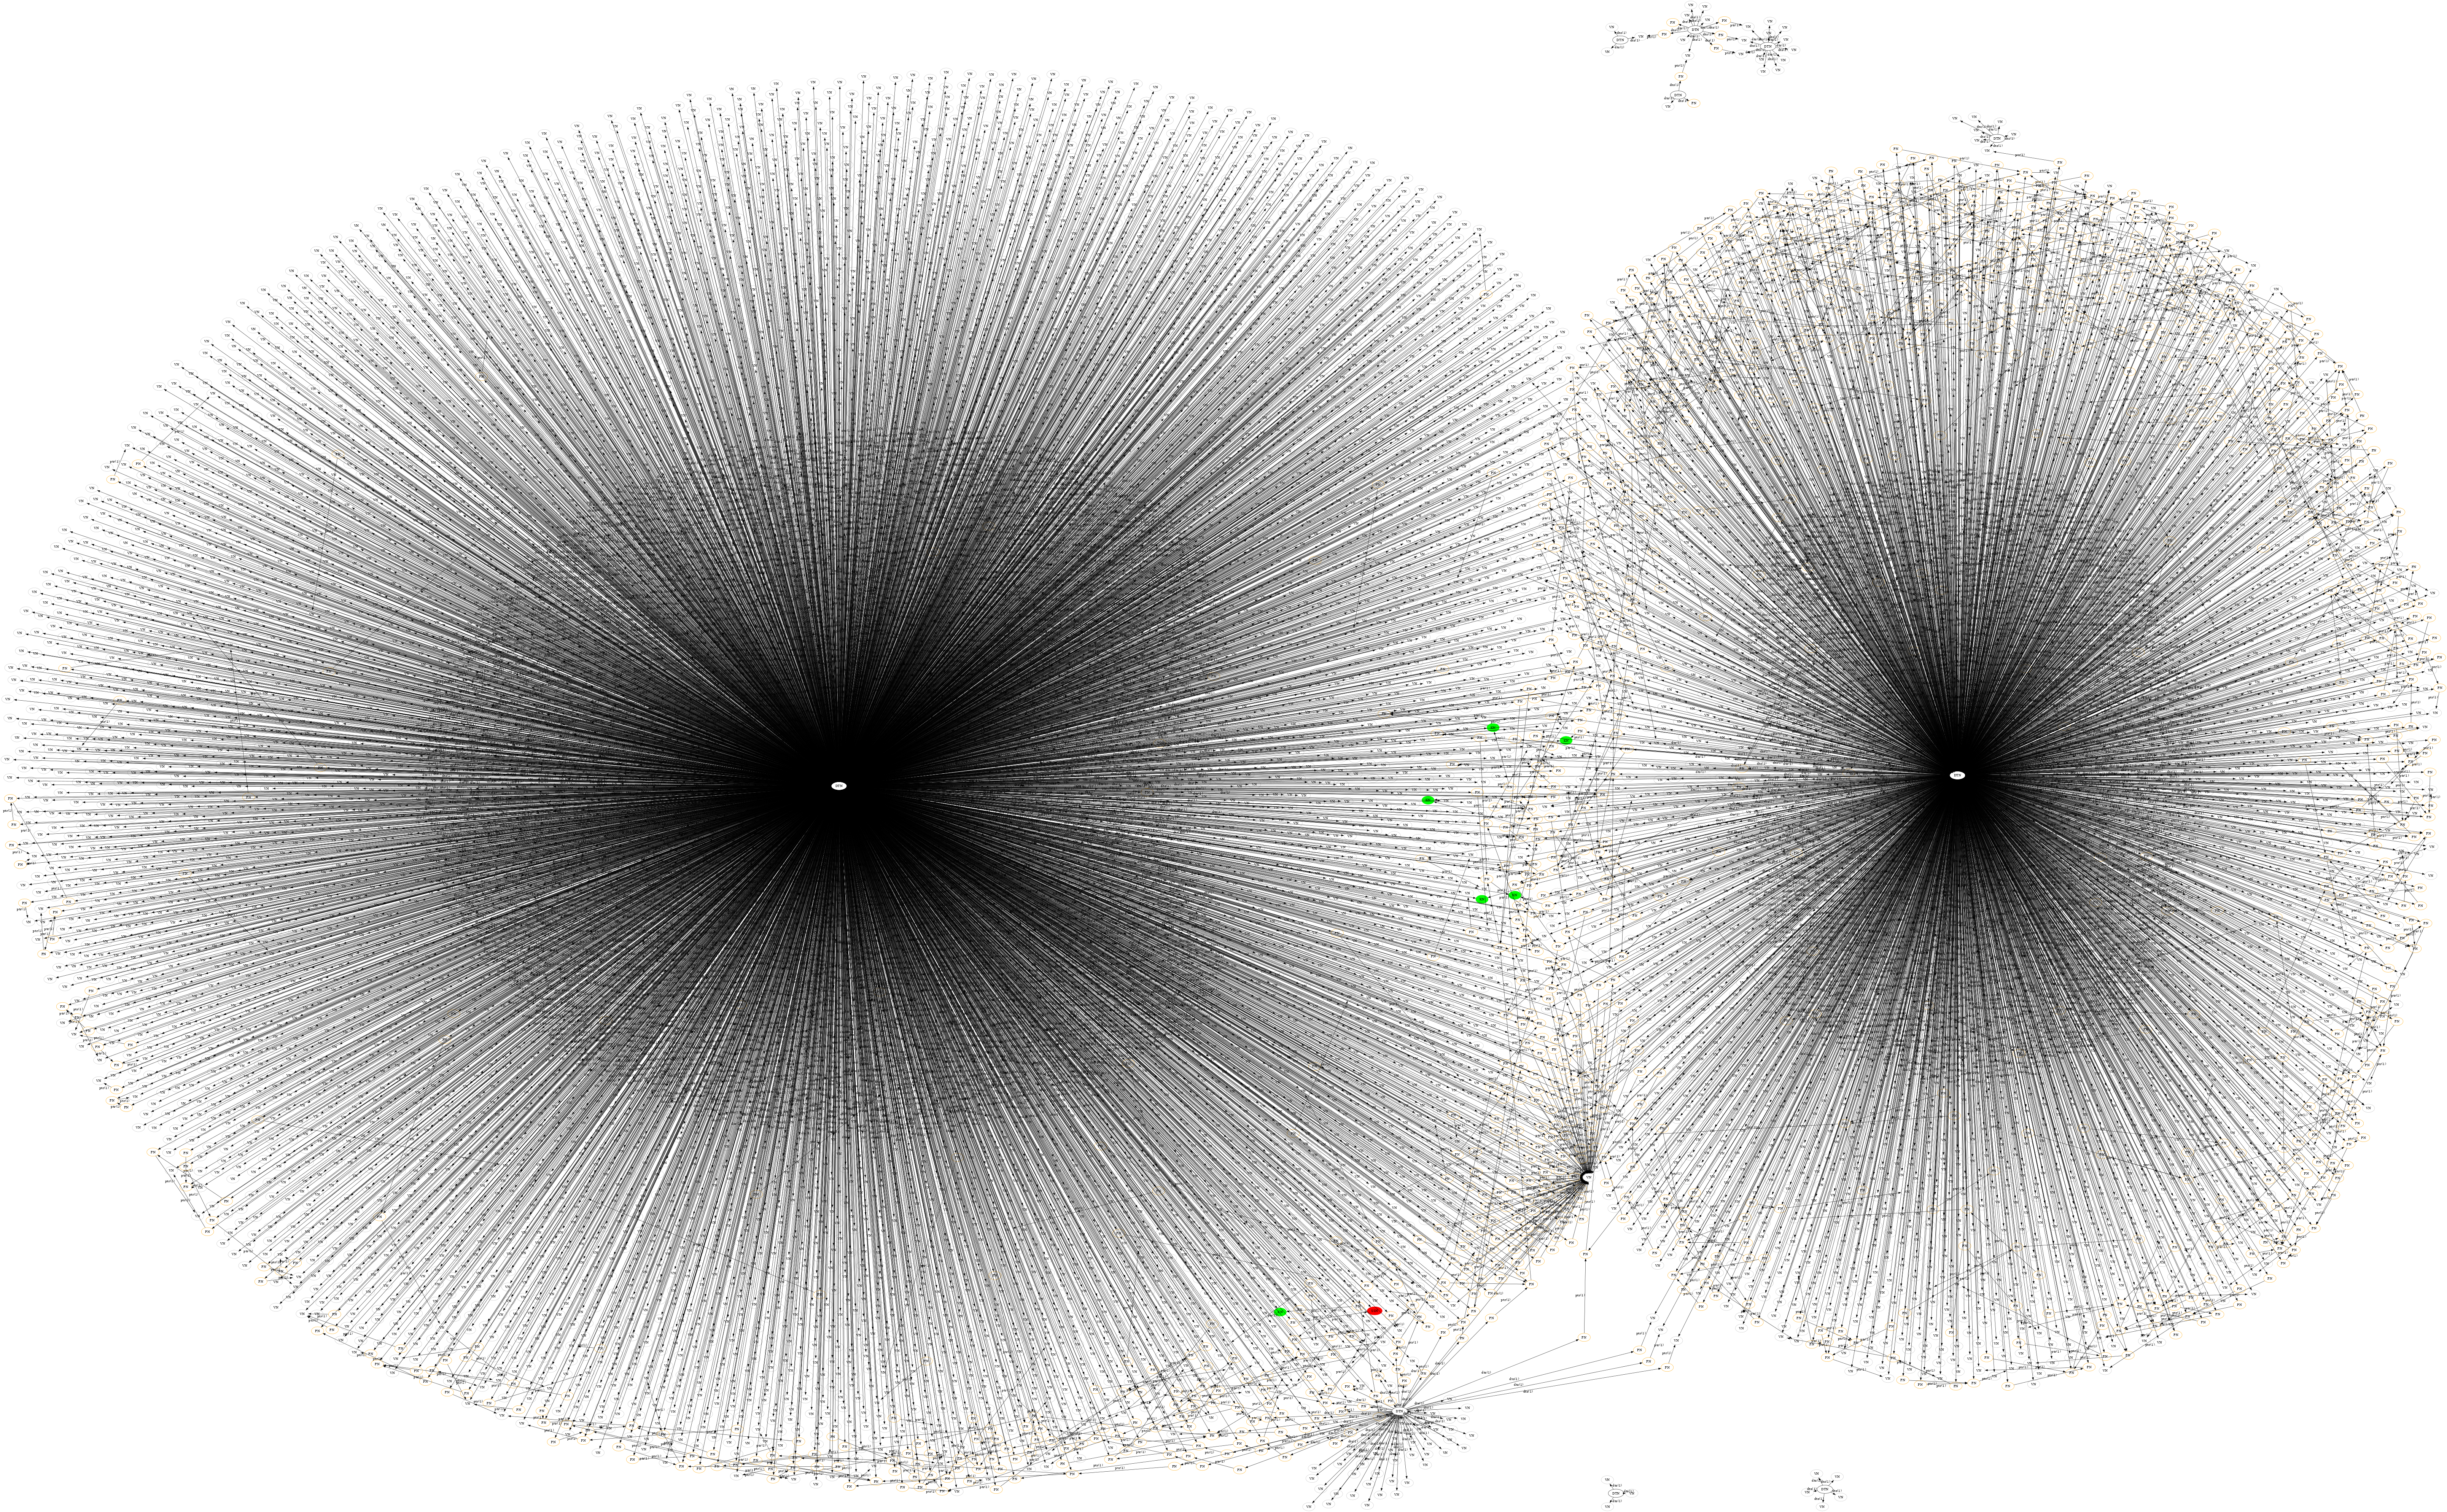
\includegraphics[width=16cm]{graphs/Training_basic_V_7_1_P1_24_17016-1643962152-heap.raw_dot_vn-sfdp.png}
    \caption{Visualization of the full memory graph generated from \textit{Training/basic/V\_7\_1\_P1/24/17016-1643962152-heap.raw}.}
\end{figure}

\begin{figure}[H]\label{appendix:mem_graph:17016-1643962152:truncated}
    \centering
    \includegraphics[width=16cm]{graphs/17016-1643962152_simplified_colored.png}
    \caption{Visualization of a truncated memory graph generated from \textit{Training/basic/V\_7\_1\_P1/24/17016-1643962152-heap.raw}. Here with real addresses.}
\end{figure}

\begin{figure}[H]\label{appendix:mem_graph:302-1644391327:full}
    \centering
    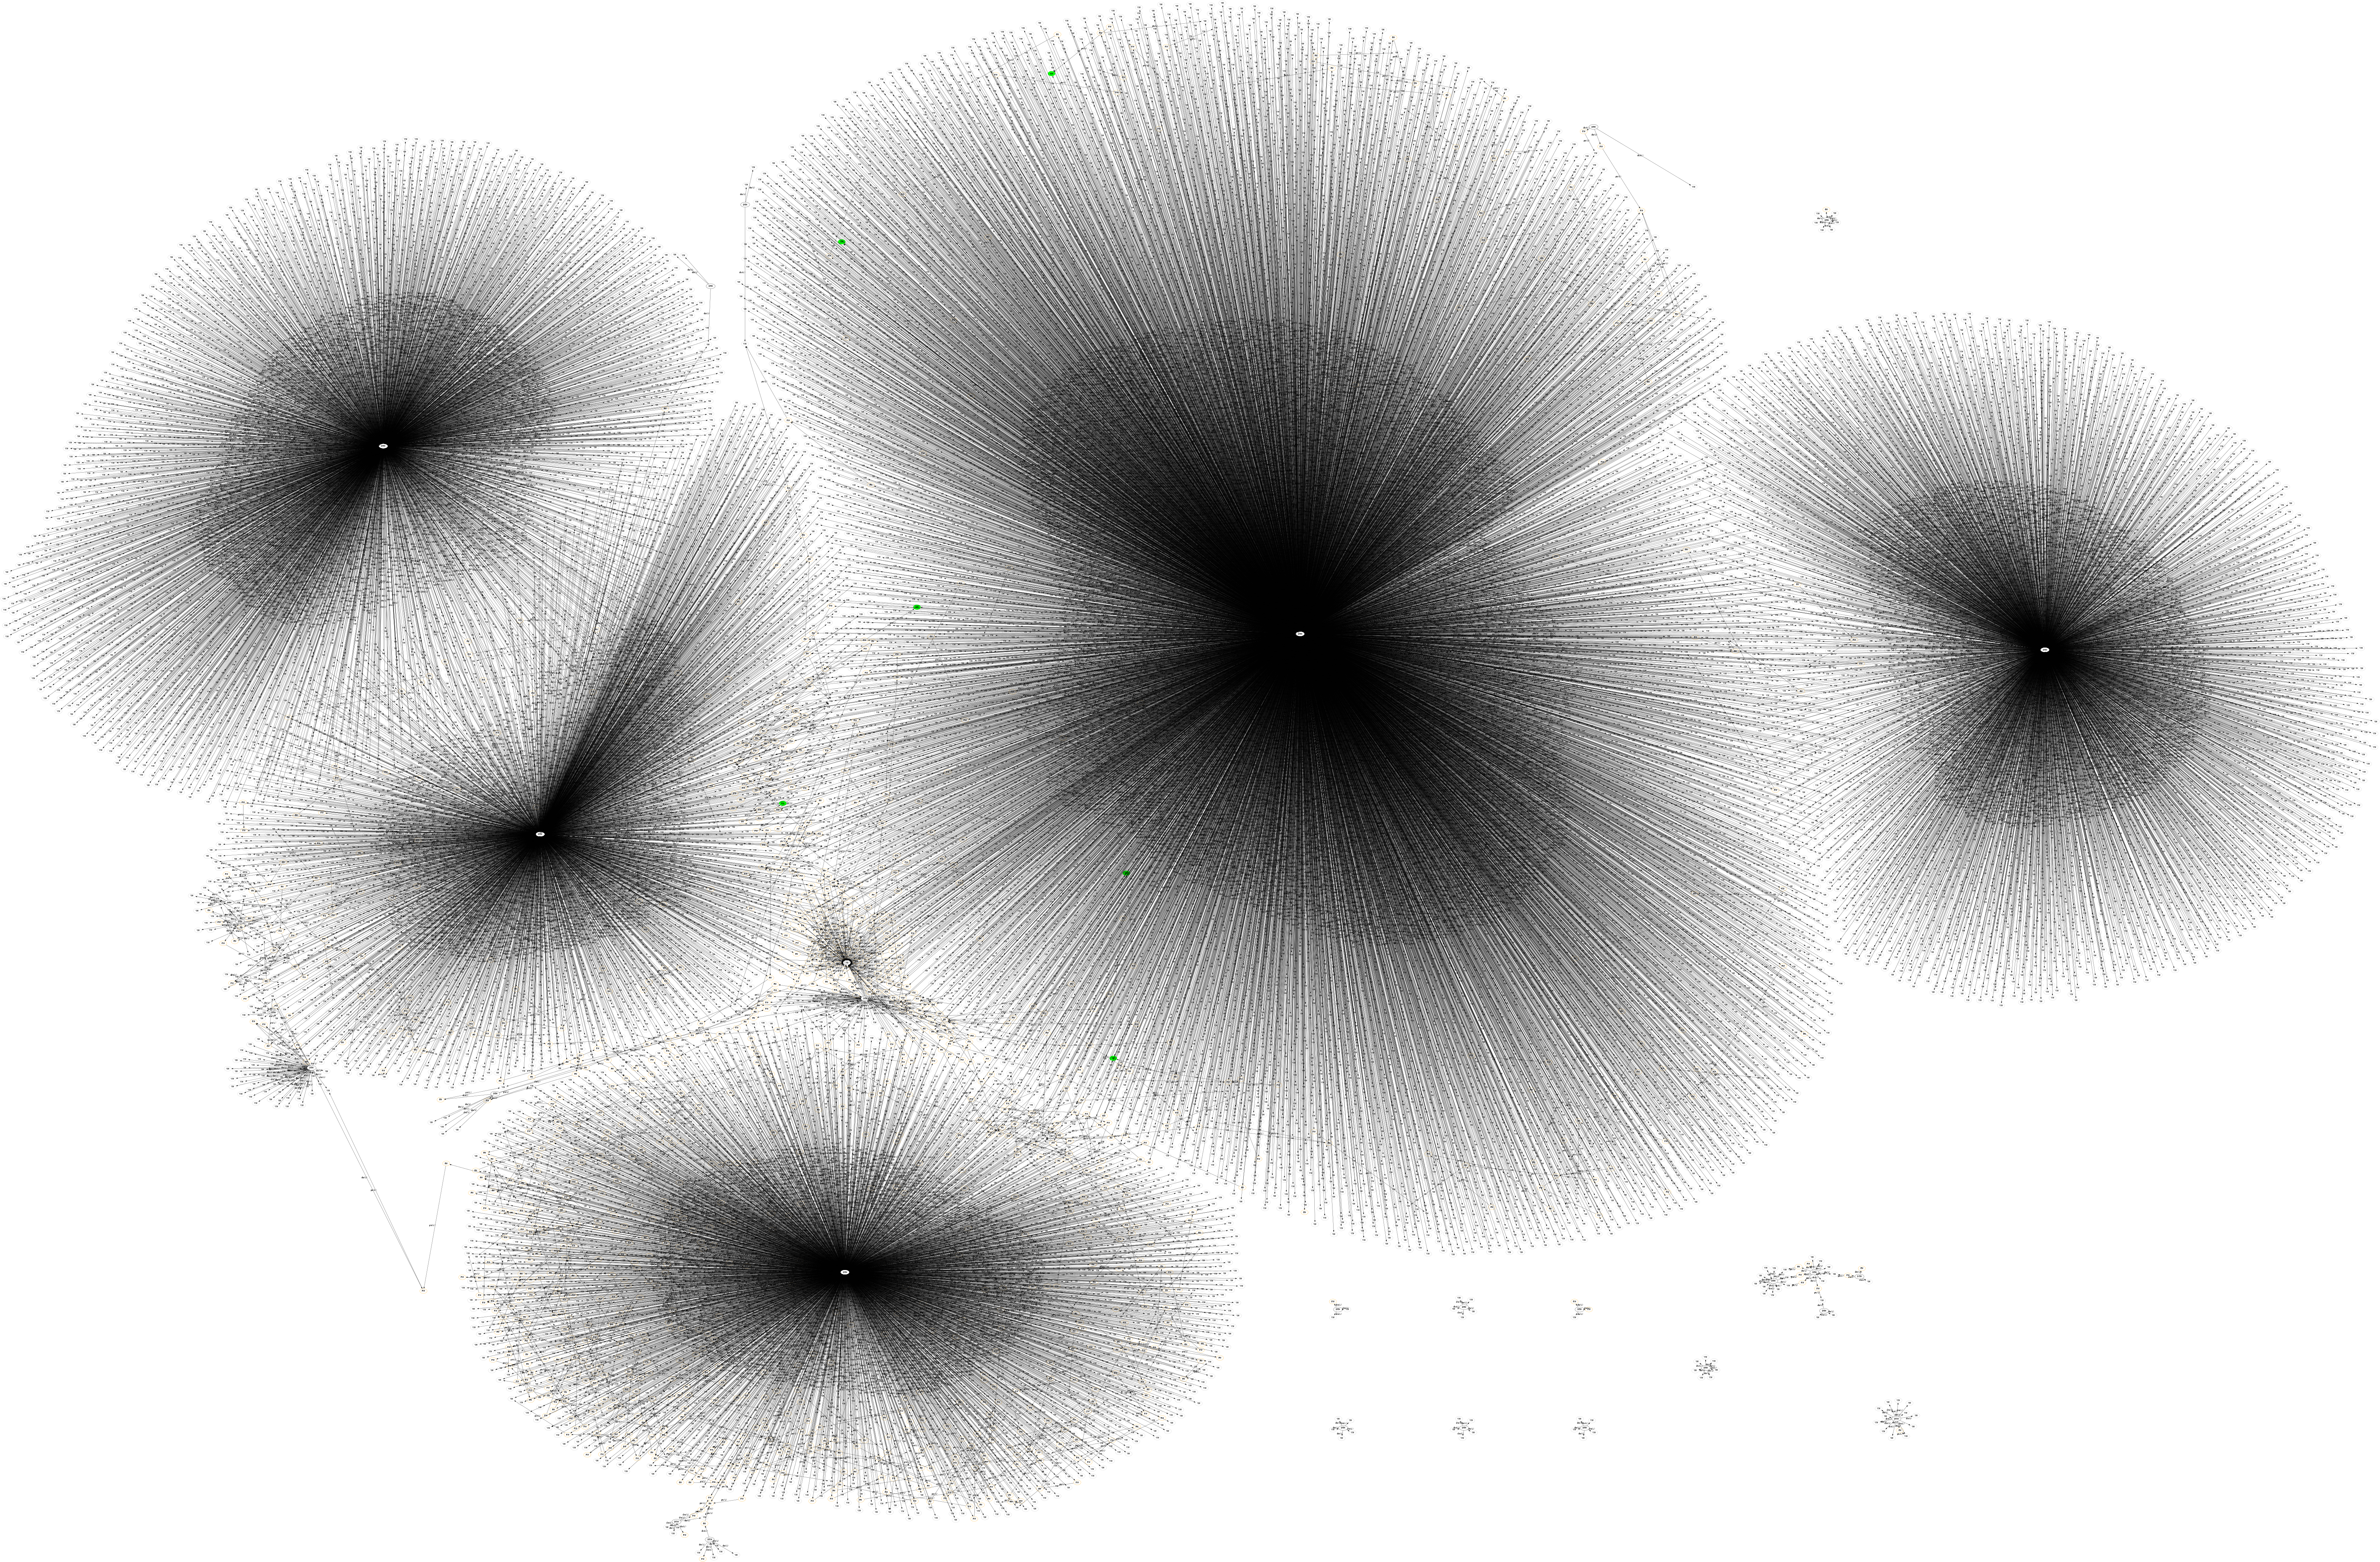
\includegraphics[width=16cm]{graphs/test_graph_from_302-1644391327_vn-sfdp.png}
    \caption{Visualization of the full memory graph generated from \textit{Training/scp/V\_7\_8\_P1/16/302-1644391327-heap.raw}.}
\end{figure}

\section{Dataset}